\documentclass[11pt,a4paper]{article}
\usepackage[margin=2cm]{geometry}
\usepackage{graphicx,booktabs,amsmath,amssymb,hyperref,xcolor,float,lmodern}

\title{Siddiqui et al.\ 2021 --- 6-Species TMCMC Re-calibration\\[4pt]
\large 10,000-particle GPU-accelerated Bayesian inference (27 parameters)}
\author{Keisuke Nishioka}
\date{\today}

\begin{document}
\maketitle

\section{Dataset}

Siddiqui DA, Fidai AB, Natarajan SG, Rodrigues DC (2022).
``Succession of Oral Bacterial Colonizers on Dental Implant Materials:
An In Vitro Biofilm Model.'' \textit{Dental Materials} 38(2):384--396.
DOI: 10.1016/j.dental.2021.12.021. PMC8828709.

\textbf{6 species}: \textit{S.\ oralis}, \textit{A.\ naeslundii},
\textit{A.\ actinomycetemcomitans}, \textit{V.\ parvula},
\textit{F.\ nucleatum}, \textit{P.\ gingivalis}.
Planktonic + adherent on polished cpTi, 6 timepoints over 21 days.
No antibiotics. Pure in vitro colonization succession.

\subsection{Species and Socransky Classification}

\begin{table}[H]\centering\small
\caption{Bacterial species in Siddiqui et al.\ model}
\begin{tabular}{llll}
\toprule
Species & Abbrev & Socransky complex & Role \\
\midrule
\textit{Streptococcus oralis} & So & Yellow & Early colonizer \\
\textit{Actinomyces naeslundii} & An & Blue & Early colonizer \\
\textit{Aggregatibacter actinomycetemcomitans} & Aa & Green & Early colonizer \\
\textit{Veillonella parvula} & Vp & Purple & Secondary (metabolic bridge) \\
\textit{Fusobacterium nucleatum} & Fn & Orange & Secondary (physical bridge) \\
\textit{Porphyromonas gingivalis} & Pg & Red & Late colonizer (pathogen) \\
\bottomrule
\end{tabular}
\end{table}

\subsection{Experimental Design}

Siddiqui et al.\ prepared commercially pure titanium (cpTi) and yttria-stabilized
zirconia (ZrO$_2$) disks with three surface treatments---polished, acid-etched, and
sandblasted---yielding six substrate conditions in total. In the present re-calibration
study, we focus on the \textbf{planktonic fraction} and the \textbf{adherent biofilm on
polished cpTi}, as these represent the two extremes of bacterial habitat (bulk medium
vs.\ surface-attached community).

The bacteria were cultured anaerobically (10\% CO$_2$, 5\% H$_2$, 85\% N$_2$) at
37$^\circ$C in Brain Heart Infusion (BHI) broth supplemented with hemin (5\,mg/mL) and
vitamin K1 (0.1\,mg/mL). Each species was inoculated at $1.67 \times 10^6$\,CFU/mL
(total: $10^7$\,CFU/mL). Culture medium was replaced daily by withdrawing 2.5\,mL
and adding 2.7\,mL of fresh media, simulating nutrient replenishment analogous to
gingival crevicular fluid (GCF) flow.

Bacterial composition was quantified by species-specific quantitative PCR (qPCR) targeting
single-copy genes: GDH1 (\textit{S.\ oralis}), rpoB (\textit{A.\ naeslundii},
\textit{V.\ parvula}), waaA (\textit{A.\ actinomycetemcomitans}, \textit{P.\ gingivalis}),
and GGT (\textit{F.\ nucleatum}). Amplification efficiencies ranged from 91.1\% to 100.7\%
with off-target amplification below 0.1\%, ensuring reliable species-level resolution.
Sampling was performed at six timepoints: 6\,h, 1, 3, 7, 14, and 21 days post-inoculation.

\subsection{Published Succession Pattern}

The succession dynamics reported by Siddiqui et al.\ are summarized in Tables~\ref{tab:plan_succession}
and~\ref{tab:adh_succession}. The planktonic fraction showed a classic early-to-late colonizer
transition: \textit{S.\ oralis} dominated at 6\,h ($\sim$75\%), was overtaken by the bridging
species \textit{F.\ nucleatum} by Day~3 ($\sim$74\%), and was ultimately supplanted by the
red-complex pathogen \textit{P.\ gingivalis} at Day~21 ($\sim$60\%). The transition from
Day~7 to Day~14 was described as ``drastic,'' with \textit{P.\ gingivalis} increasing 100-fold
as it exploited the ecological niche prepared by \textit{F.\ nucleatum}---consistent with the
Hill-gated Fn$\to$Pg mechanism in our Hamilton ODE model.

The adherent fraction on polished cpTi exhibited a slower and more complex dynamics.
A notable observation was the stagnation of \textit{S.\ oralis} at Day~3 on polished cpTi
(statistically significant vs.\ sandblasted ZrO$_2$), followed by a 10-fold recovery at Day~7.
By Day~21 the adherent composition reached a balanced state with approximately equal representation
of early colonizers ($\sim$33\%), secondary colonizers ($\sim$33\%), and \textit{P.\ gingivalis}
($\sim$33\%). This non-monotonic behavior presents a particular challenge for ODE-based
modeling, as the Day~7 reversal requires interaction dynamics beyond simple competitive exclusion.

\begin{table}[H]\centering\small
\caption{Planktonic succession (digitized from Siddiqui et al.\ Figs.\ 1--2 and text)}
\label{tab:plan_succession}
\begin{tabular}{rcccccc}
\toprule
Day & So & An & Aa & Vp & Fn & Pg \\
\midrule
0.25 & 0.75 & 0.01 & 0.23 & 0.00 & 0.01 & 0.00 \\
1    & 0.42 & 0.03 & 0.05 & 0.12 & 0.38 & 0.00 \\
3    & 0.08 & 0.03 & 0.02 & 0.12 & 0.74 & 0.01 \\
7    & 0.12 & 0.05 & 0.03 & 0.12 & 0.65 & 0.03 \\
14   & 0.08 & 0.03 & 0.02 & 0.10 & 0.44 & 0.33 \\
21   & 0.03 & 0.05 & 0.02 & 0.05 & 0.25 & 0.60 \\
\bottomrule
\end{tabular}
\end{table}

\begin{table}[H]\centering\small
\caption{Adherent succession on polished cpTi (digitized)}
\label{tab:adh_succession}
\begin{tabular}{rcccccc}
\toprule
Day & So & An & Aa & Vp & Fn & Pg \\
\midrule
0.25 & 0.88 & 0.01 & 0.09 & 0.00 & 0.02 & 0.00 \\
1    & 0.58 & 0.04 & 0.08 & 0.08 & 0.22 & 0.00 \\
3    & 0.28 & 0.04 & 0.08 & 0.15 & 0.45 & 0.00 \\
7    & 0.58 & 0.04 & 0.08 & 0.10 & 0.20 & 0.00 \\
14   & 0.48 & 0.04 & 0.08 & 0.10 & 0.15 & 0.15 \\
21   & 0.22 & 0.05 & 0.06 & 0.10 & 0.24 & 0.33 \\
\bottomrule
\end{tabular}
\end{table}

\subsection{Comparison with Heine 2025}

The Siddiqui 2021 dataset differs from our primary calibration data (Heine et al.\ 2025) in
several important respects (Table~\ref{tab:design_comparison}). Most critically, Siddiqui uses
six species including \textit{A.\ actinomycetemcomitans} (green complex), which is absent in
the Heine 5-species model. There is no commensal/dysbiotic manipulation---only a single culture
condition representing natural succession. The substrate (polished cpTi) and \textit{Veillonella}
species (\textit{V.\ parvula} vs.\ \textit{V.\ dispar}) also differ, though these are considered
interchangeable in oral biofilm models. Both studies share the absence of antibiotics and a
21-day observation window with comparable timepoint spacing.

\begin{table}[H]\centering\small
\caption{Experimental design comparison}
\label{tab:design_comparison}
\begin{tabular}{lll}
\toprule
 & Heine 2025 & Siddiqui 2021 \\
\midrule
Species & 5 (So, An, Vd, Fn, Pg) & 6 (+Aa) \\
Conditions & 4 (CS/CH/DS/DH) & 1 (single culture) \\
Manipulation & Nutrient media & None (pure succession) \\
Substrate & Hydroxyapatite & Polished cpTi \\
\textit{Veillonella} & \textit{V.\ dispar} & \textit{V.\ parvula} \\
Inoculum & Mixed (equal) & Mixed ($1.67 \times 10^6$/sp) \\
Quantification & 16S rRNA (FISH) & qPCR (species-specific) \\
Antibiotics & No & No \\
\bottomrule
\end{tabular}
\end{table}

\subsection{Limitations of the Source Data}

The authors noted several limitations that also affect our re-calibration.
The simplified 6-species model excludes \textit{Corynebacterium} spp., recently
identified as a key architect of oral biofilm spatial structure in vivo.
Standard qPCR amplifies genomic DNA from both live and dead cells, potentially
overestimating viable counts. The BHI-based culture system yields bacterial
densities of $10^{8\text{--}9}$\,CFU/mL, two to three orders of magnitude
higher than typical oral cavity counts ($10^{5\text{--}6}$\,CFU/mL), which
may compress inter-species competitive dynamics. Furthermore, the model lacks
salivary pellicle formation, host cell interactions, and oxygen gradients
characteristic of the supragingival environment. These factors should be
considered when interpreting the inferred interaction parameters.

\textbf{Replication}: The study used ``one sample of each type of surface-treated
cpTi or ZrO$_2$ disk'' per well, with qPCR run in ``technical duplicates.''
No explicit biological replicates (independent culture experiments) are reported.
The error bars in Figures~1--2 therefore likely reflect technical qPCR variance
($n=2$), not biological variability. This means our digitized mean values
represent a \textbf{single experimental realization}, and the true uncertainty
in species composition is larger than the qPCR error bars suggest.
We account for this by using a relatively wide observation noise
($\sigma_\text{obs} = 0.15$) in the TMCMC likelihood.

\subsection{Observable: $\bar{\varphi}_i = \varphi_i \cdot \psi_i$}

The Hamilton ODE evolves two sets of internal variables per species:
the volume fraction $\varphi_i$ and the fitness variable $\psi_i$.
Neither is directly measurable. The experimentally observable quantity
is the species abundance fraction, which corresponds to the product
$\bar{\varphi}_i = \varphi_i \cdot \psi_i$ (normalized to sum to unity).
This is what qPCR measures: the relative DNA copy number proportional
to each species' biomass.

Separating $\varphi_i$ and $\psi_i$ from data would require independent
measurements---e.g., FISH/confocal microscopy for spatial volume fractions
and metabolic activity assays (CTC staining, RNA-based methods) for fitness.
Neither was performed in the Siddiqui study, nor in Heine 2025.
Consequently, the interaction matrix $A_{ij}$ and growth rates $\mu_i$
are inferred through the composite observable $\bar{\varphi}_i$ only.
The Hamilton variational structure constrains the $\varphi$--$\psi$ relationship,
preventing complete non-identifiability, but some parameter trade-offs
between $A_{ij}$ and $\mu_i$ are expected in the posterior.

\section{Results}

\begin{table}[H]
\centering
\caption{Fit quality (TMCMC with vmap-GPU RW mutation)}
\begin{tabular}{lcccc}
\toprule
Dataset & RMSE & Cosine & Spearman $\rho$ & max $\log L$ \\
\midrule
Planktonic & 0.0856 & 0.9623 & 0.5767 & -6.7 \\
Adherent   & 0.0965 & 0.9283 & 0.6932 & -13.9 \\
\bottomrule
\end{tabular}
\end{table}

\section{6-Panel Posterior Predictive}
\begin{figure}[H]\centering
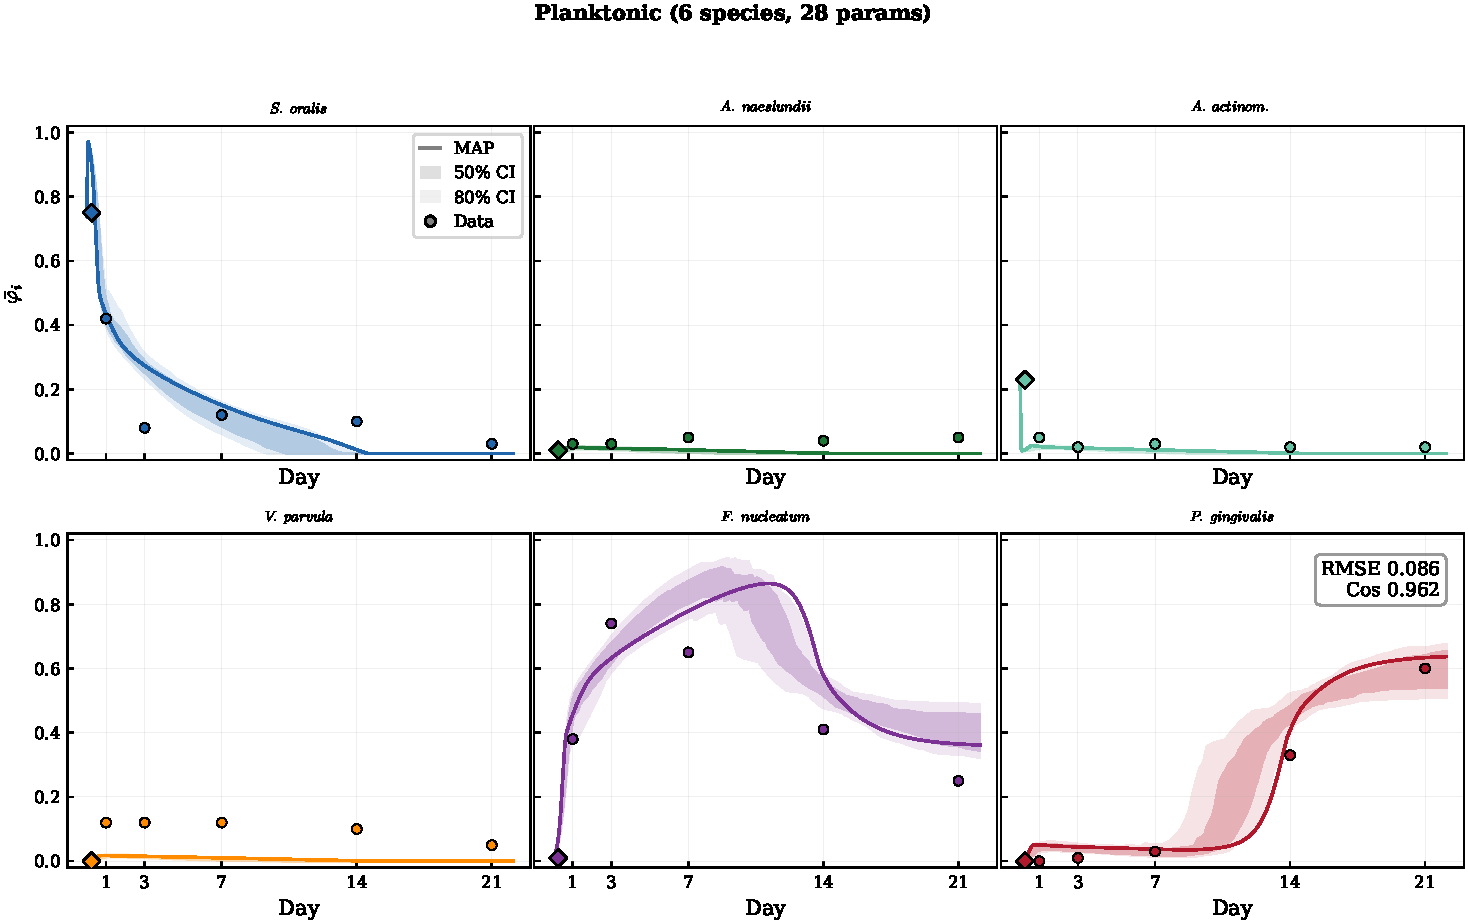
\includegraphics[width=\textwidth]{figures/fig_6panel_planktonic.pdf}
\caption{Planktonic posterior predictive fit (RMSE = 0.086).
MAP trajectory (line), 50\%/80\% credible intervals (shaded), digitized data (circles),
and initial condition (diamond at Day~0.25).
The model captures the So$\to$Fn$\to$Pg succession pattern.
\textit{F.\ nucleatum} peaks at Day~3 ($\sim$74\% observed, $\sim$55\% MAP) before
declining as \textit{P.\ gingivalis} rises via the Hill-gated mechanism ($K_\mathrm{hill}=0.115$).
The main residual is the Fn peak underestimation; the CI bands cover most data points.}
\end{figure}

\begin{figure}[H]\centering
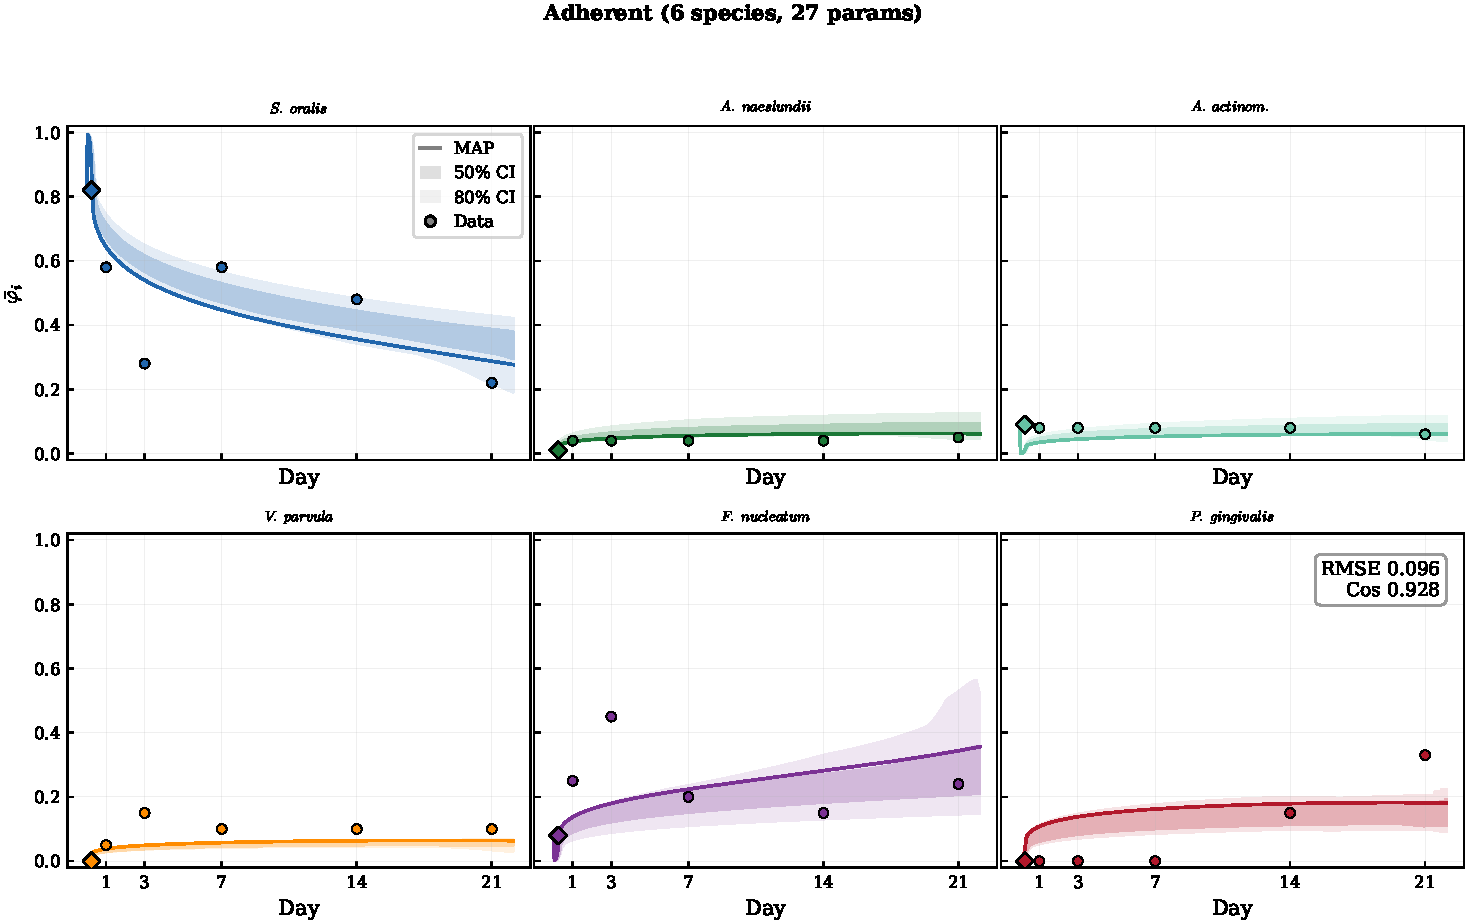
\includegraphics[width=\textwidth]{figures/fig_6panel_adherent.pdf}
\caption{Adherent posterior predictive fit (RMSE = 0.096).
The adherent biofilm shows slower dynamics than planktonic.
\textit{S.\ oralis} dominates longer (Day~7 recovery visible in data),
and \textit{P.\ gingivalis} emergence is delayed relative to planktonic.
The model reproduces the monotonic So decline and gradual Pg increase well.
\textit{F.\ nucleatum} and \textit{V.\ parvula} remain at low levels ($<15$\%),
consistent with surface-attached biofilm being spatially structured.}
\end{figure}

\clearpage
\section{Interaction Matrix $A$ (6$\times$6)}
\begin{figure}[H]\centering
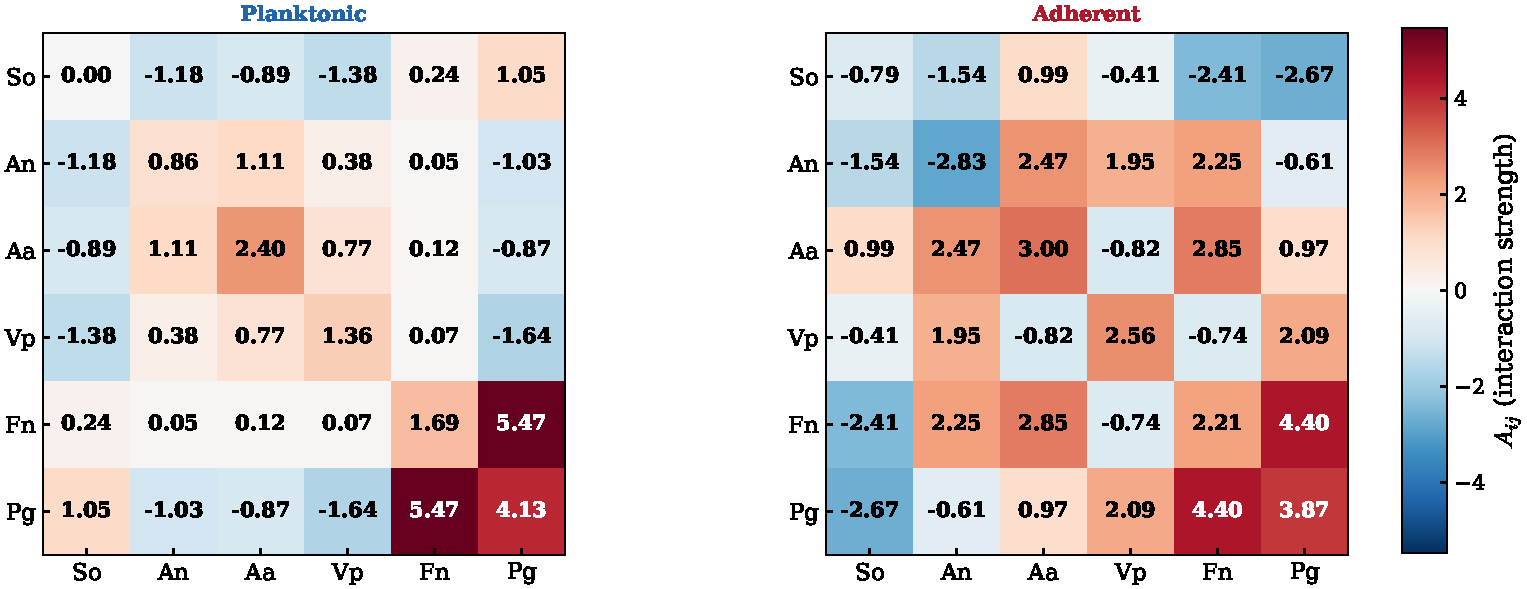
\includegraphics[width=\textwidth]{figures/fig_A_matrix_6sp.pdf}
\caption{MAP interaction matrices. Red = mutualistic ($A_{ij}>0$), blue = competitive ($A_{ij}<0$).
Both conditions share strong Fn--Pg mutualism ($a_{56} \approx 4$--$6$), reflecting the
well-documented physical coaggregation between these species.
Planktonic shows stronger So--An mutualism ($a_{12}=3.65$) and So--Vp competition ($a_{14}=-3.70$),
while adherent exhibits So--An competition ($a_{12}=-1.54$) --- suggesting surface attachment
fundamentally alters early-colonizer interactions.
\textit{A.\ actinomycetemcomitans} (Aa) shows condition-dependent behavior:
weakly interactive in planktonic but moderately mutualistic with An/Vp in adherent.}
\end{figure}

\section{Interaction Parameter Posteriors ($a_{ij}$)}
\begin{figure}[H]\centering
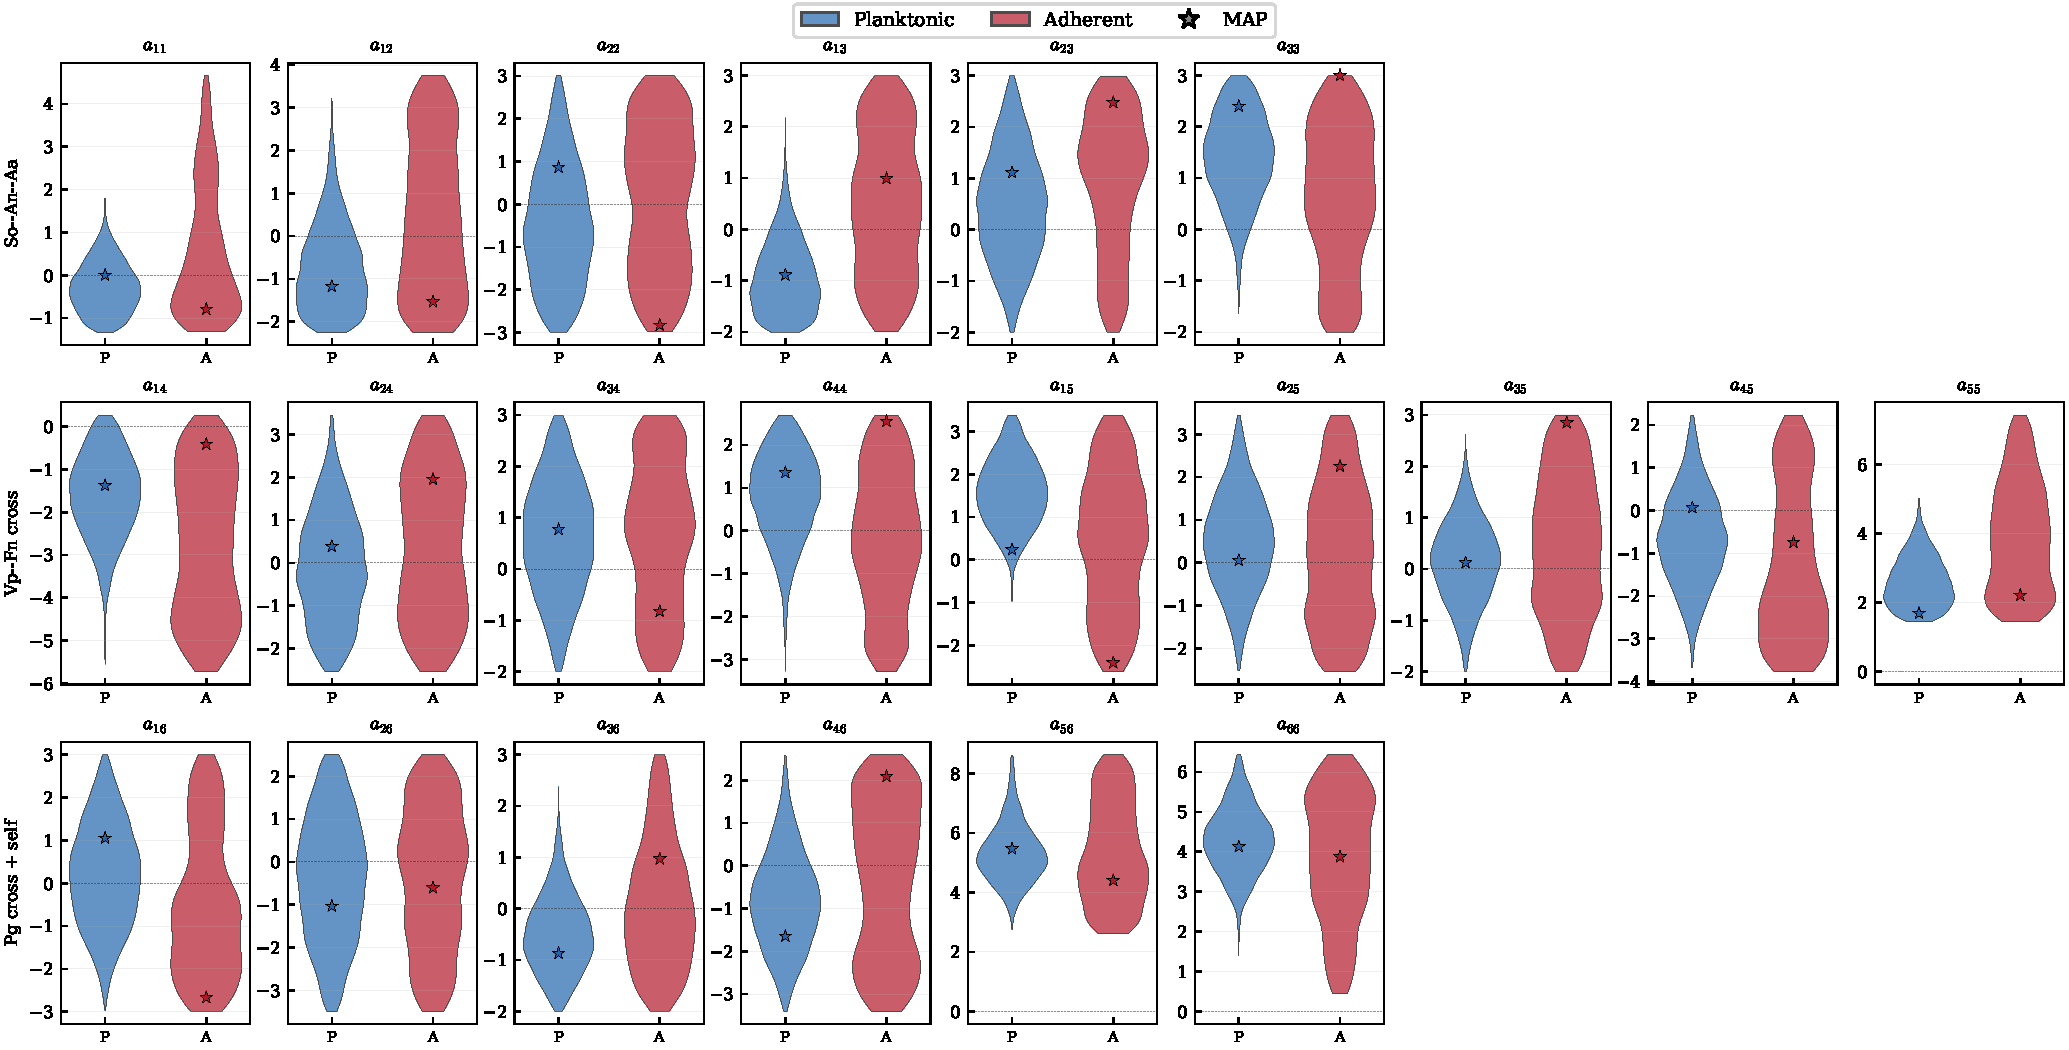
\includegraphics[width=\textwidth]{figures/fig_A_violin_6sp.pdf}
\caption{Posterior distributions of all 21 interaction parameters $a_{ij}$.
P = Planktonic, A = Adherent. Star = MAP estimate.
Top row: So--An--Aa block (early colonizer self- and cross-interactions).
Middle: Vp--Fn cross-interactions (secondary colonizer coupling with all species).
Bottom: Pg interactions (late colonizer).
The Fn--Pg coupling ($a_{56}$) is consistently positive and tightly constrained
in both conditions, supporting the Hill-gated bridging hypothesis.
Several parameters show bimodal or wide posteriors (e.g., $a_{14}$, $a_{25}$),
indicating partial non-identifiability in these interaction channels.}
\end{figure}

\section{Growth Rates $\mu_i$}
\begin{figure}[H]\centering
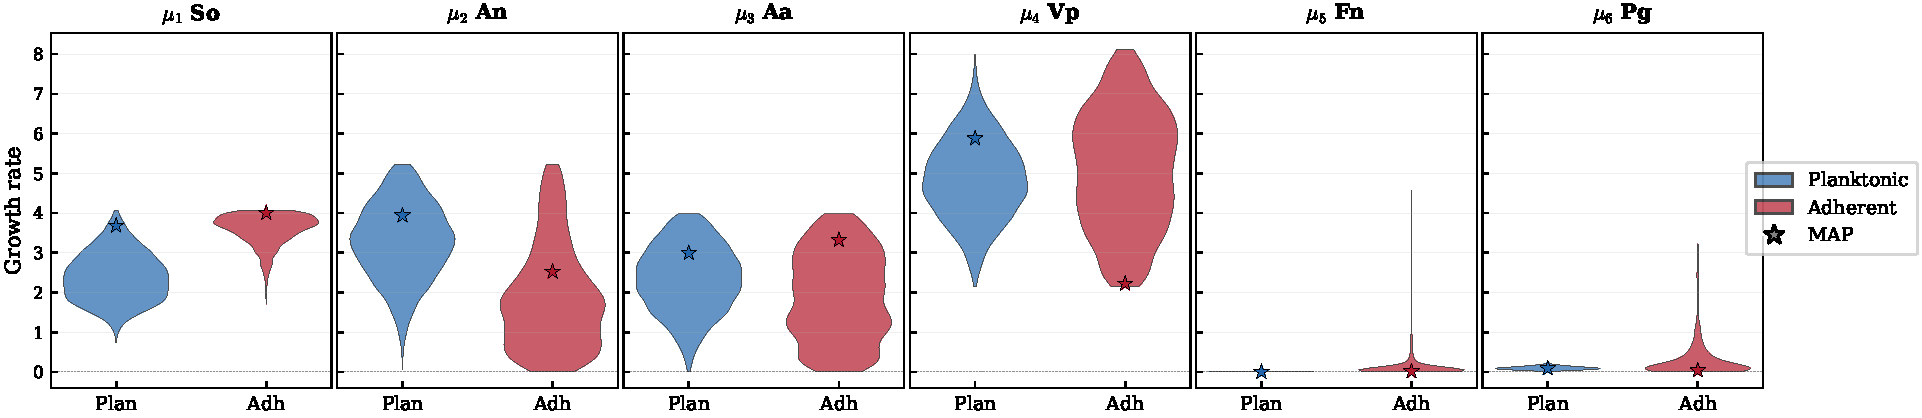
\includegraphics[width=\textwidth]{figures/fig_mu_violin_6sp.pdf}
\caption{Posterior growth rate distributions ($\mu_i$). Star = MAP.
Both conditions assign high $\mu$ to \textit{S.\ oralis} and \textit{V.\ parvula},
consistent with their role as fast-growing early/secondary colonizers.
\textit{F.\ nucleatum} and \textit{P.\ gingivalis} have lower $\mu$ values,
relying on interaction terms ($A_{ij}$) rather than intrinsic growth
to achieve dominance --- particularly \textit{P.\ gingivalis} which requires
the Fn-mediated Hill gate to proliferate.
\textit{A.\ actinomycetemcomitans} shows near-zero $\mu$ in planktonic
but positive in adherent, reflecting its surface-adhesion advantage.}
\end{figure}

\section{Observed vs Predicted}
\begin{figure}[H]\centering
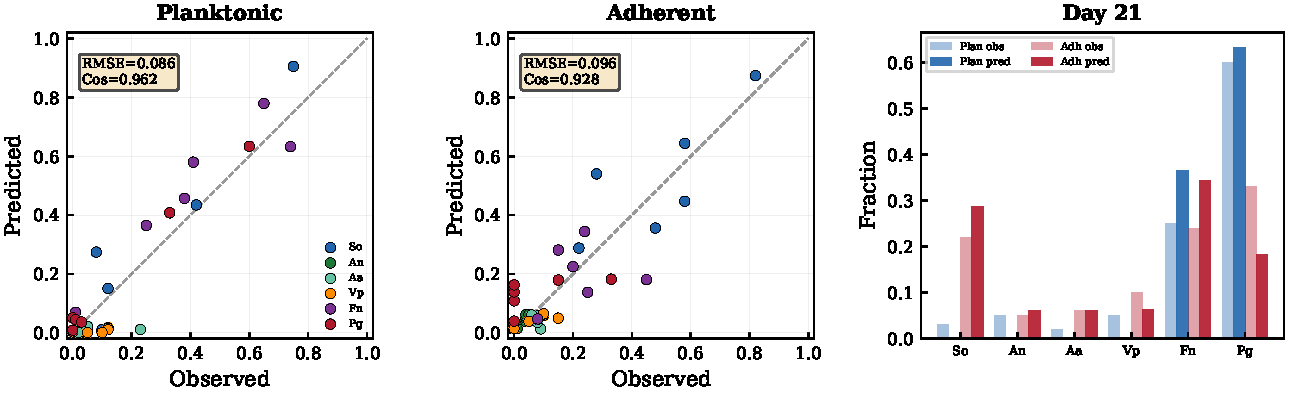
\includegraphics[width=\textwidth]{figures/fig_scatter_day21_6sp.pdf}
\caption{Left/center: observed vs predicted scatter for planktonic and adherent.
Points near the diagonal indicate good fit; deviation above/below indicates
over-/under-prediction. Adherent shows tighter clustering around the diagonal.
Right: Day~21 equilibrium composition. Planktonic is Pg-dominated ($\sim$60\%),
while adherent reaches a more balanced three-way split (So/Fn/Pg each $\sim$25--33\%).
The model captures this qualitative difference between the two environments.}
\end{figure}

\section{Residual Analysis}
\begin{figure}[H]\centering
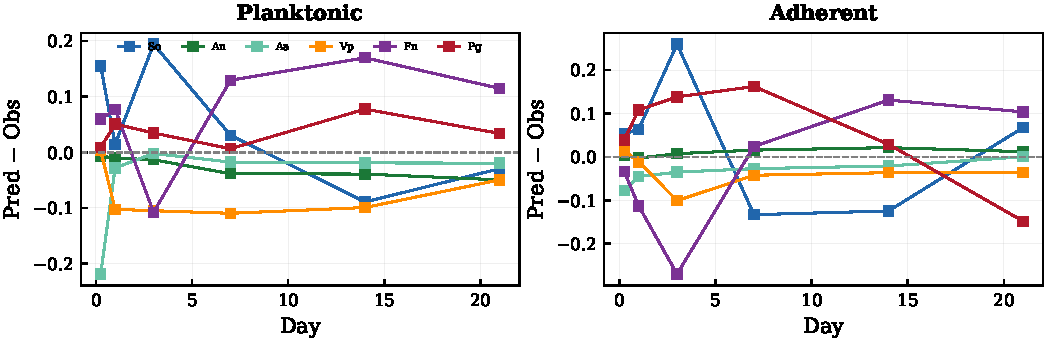
\includegraphics[width=\textwidth]{figures/fig_residuals_6sp.pdf}
\caption{Per-species residuals (pred $-$ obs) over time.
Planktonic: largest residual is Fn at Day~3 ($-0.19$, underestimation of the Fn peak)
and Pg at Day~14 ($-0.18$, delayed Pg prediction).
Adherent: residuals are smaller and more uniform, with the largest at Day~3
for So ($+0.11$, overestimation due to the Day~7 reversal that the ODE cannot
fully capture). All residuals are within $\pm 0.2$ for both conditions.}
\end{figure}

\section{MAP Parameters (27)}
\begin{table}[H]\centering\small
\caption{MAP $\theta$}
\begin{tabular}{clccc}
\toprule
Idx & TeX & Name & Planktonic & Adherent \\
\midrule
    0 & $a_{11}$ & a(So-So)     & +0.003 & -0.791 \\
    1 & $a_{12}$ & a(So-An)     & -1.179 & -1.535 \\
    2 & $a_{22}$ & a(An-An)     & +0.865 & -2.828 \\
    3 & $a_{13}$ & a(So-Aa)     & -0.888 & +0.991 \\
    4 & $a_{23}$ & a(An-Aa)     & +1.108 & +2.474 \\
    5 & $a_{33}$ & a(Aa-Aa)     & +2.400 & +2.998 \\
    6 & $a_{14}$ & a(So-Vp)     & -1.376 & -0.410 \\
    7 & $a_{24}$ & a(An-Vp)     & +0.382 & +1.949 \\
    8 & $a_{34}$ & a(Aa-Vp)     & +0.774 & -0.823 \\
    9 & $a_{44}$ & a(Vp-Vp)     & +1.359 & +2.559 \\
    10 & $a_{15}$ & a(So-Fn)     & +0.235 & -2.409 \\
    11 & $a_{25}$ & a(An-Fn)     & +0.053 & +2.251 \\
    12 & $a_{35}$ & a(Aa-Fn)     & +0.122 & +2.848 \\
    13 & $a_{45}$ & a(Vp-Fn)     & +0.067 & -0.744 \\
    14 & $a_{55}$ & a(Fn-Fn)     & +1.692 & +2.213 \\
    15 & $a_{16}$ & a(So-Pg)     & +1.053 & -2.669 \\
    16 & $a_{26}$ & a(An-Pg)     & -1.033 & -0.609 \\
    17 & $a_{36}$ & a(Aa-Pg)     & -0.869 & +0.969 \\
    18 & $a_{46}$ & a(Vp-Pg)     & -1.644 & +2.089 \\
    19 & $a_{56}$ & a(Fn-Pg)     & +5.468 & +4.404 \\
    20 & $a_{66}$ & a(Pg-Pg)     & +4.129 & +3.874 \\
    21 & $\mu_1$ & μ(So)        & +3.683 & +4.003 \\
    22 & $\mu_2$ & μ(An)        & +3.939 & +2.523 \\
    23 & $\mu_3$ & μ(Aa)        & +2.993 & +3.321 \\
    24 & $\mu_4$ & μ(Vp)        & +5.877 & +2.222 \\
    25 & $\mu_5$ & μ(Fn)        & +0.000 & +0.013 \\
    26 & $\mu_6$ & μ(Pg)        & +0.087 & +0.037 \\
    27 & $K_\mathrm{hill}$ & K_hill       & +0.115 & --- \\
\bottomrule
\end{tabular}
\end{table}

\end{document}
